%Copyright 2008 Sarah LEVY (sarah.levy@epfl.ch)
%
%This file is part of ParaViewHelper.
%
%ParaViewHelper is free software: you can redistribute it and/or modify
%it under the terms of the GNU General Public License as published by
%the Free Software Foundation, either version 3 of the License, or
%(at your option) any later version.
%
%ParaViewHelper is distributed in the hope that it will be useful,
%but WITHOUT ANY WARRANTY; without even the implied warranty of
%MERCHANTABILITY or FITNESS FOR A PARTICULAR PURPOSE.  See the
%GNU General Public License for more details.
%
%You should have received a copy of the GNU General Public License
%along with ParaViewHelper.  If not, see <http://www.gnu.org/licenses/>.

\chapter{How to use ParaViewHelper, a tutorial}

\section{Install Paraview}
	\begin{enumerate}
	\item Install Paraview
		\begin {itemize}
		\item Download Paraview on the website www.paraview.org 
		\\ You can also find the latest binary version of Paraview for 64 bits there: http://lsmspc22.epfl.ch/spip.php?article11
		\item Move the compressed file where you want it to be. The directory path is \$PARAVIEW\_HOME.
		\item Untar the downloaded version : tar xvfz paraview-3.2.0-Linux-x86\_em64.tar.gz
		\end {itemize}
	\item Download the script that generates movies: http://lsmspc22/apps/generatePVD.pl 
	\\Put it in PARAVIEW\_HOME/bin
	\item Update your bashrc : echo export PATH=\$PATH/\$PARAVIEW\_HOME/bin $>>\sim$/.bashrc
	\end{enumerate}

\section{Modify your code}
ParaViewHelper is a library of functions that can be called from a C code to generate paraview output files. If you want to use it, follow these steps. You can find the details to use coorectly each function in the paragraph \ref{libuse}.
	\begin{enumerate}
	\item Declare the global variable \emph{PHelper *handle;}

	\item Include ParaViewHelper library: \\ \emph{\#include "dumper\_paraview\_C\_wrapper.h"} 

	\item Create the function that initializes ParaViewHelper: 
		\begin{tabbing}
		\hspace{15mm} \=void Init\_Paraview()\\
		\>\{\\
		\>handle = getNewHandle();\\
		\>SetPoints(handle,coordinates,spatial\_dimension,nodes,"bar");\\
		\>SetConnectivity(handle,connectivity,TRIANGLE2,elements,FORTRAN\_MODE);\\
		\>SetMode(handle,TEXT);\\
		\>SetPrefix(handle,"paraview\_files");\\
		\>Init(handle);\\
		\>\}
		\end{tabbing}

	Call \emph{Initialize\_Paraview()} in your main.c after having allocated space for arrays ( \emph{coordinates} and \emph{connectivity} in the example).

	\item Create the function that generates your output files:
		\begin{tabbing}
		\hspace{15mm} \=void Plot\_Paraview()\\
		\>\{\\
		\>SetPoints(handle,coordinates,spatial\_dimension,nodes,"bar");\\
		\>SetConnectivity(handle,connectivity,TRIANGLE2,elements,FORTRAN\_MODE);\\
		\>AddNodeDataField(handle,displacements,spatial\_dimension,"displacements");\\
		\>SetEmbeddedValue(handle,"displacements",1);\\
		\>AddElemDataField(handle,stresses,strain\_dimension,"stresses");\\
		\>Dump(handle);\\
		\>\}
		\end{tabbing}
	Call \emph{Plot\_Paraview()} when you want to display \emph{displacements} or \emph{stresses}.


	\item Change your makefile. Here is one of my makefile for SimulPack, you can adapt it to your project.

	\begin{tabbing}
	\hspace{15mm} \= PARAVIEWHELPER\_HOME= /home/slevy/ParaviewHelper/\\
	\>BINDIR = . \\
	\>PROJECT = adlib\\
	\>CASE   = exe\\
	\>PROJ\_BIN = \$(BINDIR)/\$(CASE)\\
	\>LIBDIR  = \$(SIMULPACK\_HOME)/lib\$(OPTIM)\\
	\>INCDIR =   -I\$(SIMULPACK\_HOME)/adlib -I\${PARAVIEWHELPER\_HOME}/src\\
	\>CFLAGS =  \$(OPTIM) \$(INCDIR) -lstdc++\\
	\>FFLAGS =  \$(OPTIM) \$(INCDIR)\\
	\>LDFLAGS = \$(OPTIM) \$(INCDIR)\\
	\>SRCC = $\backslash$\\
	\> 	 \hspace{1cm}main.c\\
	\>SUFFIXES = .o .c\\
	\>.SUFFIXES: \$(SUFFIXES)\\
	\>OBJC    = \$(SRCC:.c=.o)\\
	\>SRC = \$(SRCC)\\
	\>OBJ = \$(OBJC)\\
	\>ADLIB\_LIBS = \$\{addprefix \$(LIBDIR)/\$(PROJECT)/,mechanics.a mesher2d.a \\
	\> \hspace{1cm} utils.a fem.a materials.a libmyutils.a\} TECPLOT\_LIB = /usr/tec100/lib/tecio64.a\\
	\>LIBRARIES = \$(ADLIB\_LIBS) \$(TECPLOT\_LIB)\\
	\>.c.o:\\
	\>	\hspace{1cm}\$(CC) -c  \$(CFLAGS) \$(INC) \$(DEF) \$$<$\\
	\>\$(PROJ\_BIN): \$(OBJ)\\
	\>       \hspace{1cm} \$(CC) \$(CFLAGS) \$(OBJ) -o \$(PROJ\_BIN) \$(FOR\_OBJ) \$(LIBRARIES) -lm -lg2c -Wall -L\\
        \>\${PARAVIEWHELPER\_HOME}/src -lParaviewHelper -Wl,-rpath \${PARAVIEWHELPER\_HOME}/src -lz\\
	\>clean:\\
	\>        \hspace{1cm} -rm -f *.o exe;\\
	\end{tabbing}

	\end{enumerate}


\section{Use Paraview}
	\begin{enumerate}
	\item{Generate and read output files:}
		\begin{itemize}
		\item You can now run your executable. 
		\item It generates some files into the directory paraview\_files that you should have previously created. Notice that there are two different types of files \emph{bar\_pvf0000.proc0000.vtu} and \emph{bar\_pvf0000.pvtu} that are the same if you code is not parallelized. 
		\item Once paraview opened (type \emph{paraview} in you console ), load for example \emph{bar\_pvf0000.proc0000.vtu}. Click on \emph{Apply}, green button on your main screen.\\\\
		\begin{center}
		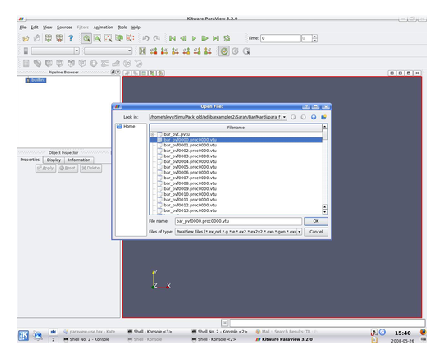
\includegraphics{snap1.eps}\\
		\vspace{0.5cm} 
		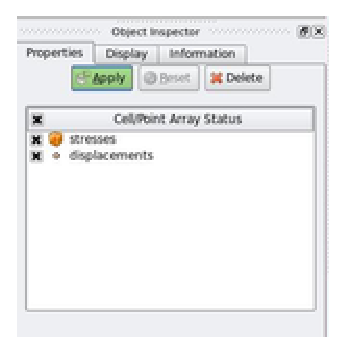
\includegraphics{snap6.eps}\\
		\vspace{0.5cm}
		\end{center}
		\item By default, \emph{surface} which is situated in the tool bar, is selected. You might prefer \emph{Surface with edges} that displays the mesh.\\
		\item If you want to see the displacements, switch \emph{Solid Color} in the tool bar to \emph{displacements}.\\
		\begin{center}
\includegraphics{snap7.eps}\\\end{center}
		\item On the left side of the main screen,\emph{Display} gives all the options to customize your screen. For instance, you can click on \emph{Edit Color Map} to display the legend.\\
		\begin{center}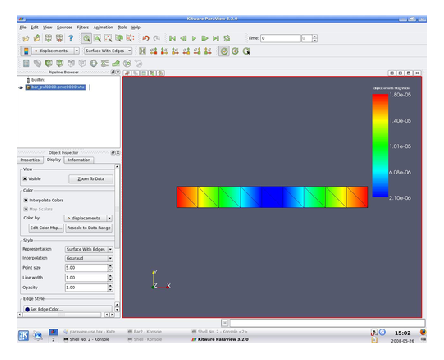
\includegraphics{snap2.eps}\\\end{center}
		\end{itemize}
	
	\item{Generate and read a movie}
		\begin{itemize}
		\item Type on your console \emph{generatePVD.pl directory bar >name\_movie.pvd} , where directory indicates the location of your vtu files. If you change one of you .vtu files, you don't need to recreate name\_movie.pvd.
		\item Open paraview. Open name\_movie.pvd. Don't forget to click on the green \emph{Apply} button.Choose the field you want to display, display the color map and play the movie).
		\item If you want to export the movie as a .avi file,
			\begin{itemize}
			\item first, generate a list of .jpg files using \textit{"Save animation"} in the File menu.
			\item then, use this command to turn the .jpg files into a .avi movie \textit{"mencoder "mf://*.jpg" -mf fps=6:type=jpg -ovc lavc -lavcopts vcodec=msmpeg4v2 -of avi -o movie.avi"}
			\end{itemize}
		\end{itemize}


	\end{enumerate}


\vspace{1.5cm}
These are the basics to generate paraview files and movie. If you are willing to improve your skills on paraview, you can refer to the User Manual book which is in our library!

